\documentclass[letter,12pt]{article}


\usepackage[english]{babel}

\usepackage{fancyhdr}


\usepackage{graphicx}
\usepackage{amsmath}
\usepackage{amssymb}
\usepackage[latin1]{inputenc}
\usepackage{fancybox}
\usepackage{amsfonts}
\usepackage{bbold}
\usepackage{textcomp}


\setlength{\oddsidemargin}{0in}
\setlength{\evensidemargin}{0in}
\setlength{\textwidth}{16.1 cm}
\setlength{\topmargin}{-15mm}
\setlength{\textheight}{22cm}
\setlength{\parindent}{0cm}


\newcommand{\sv}{\underline}
\newcommand{\Sig}{\boldsymbol{\sigma}}
\newcommand{\K}{\boldsymbol{K}}
\newcommand{\Eps}{\boldsymbol{\varepsilon}}
\newcommand{\intener}{\mathcal{E}}


% --------------------------------------------------------------------------------------
% - definition des notations
% --------------------------------------------------------------------------------------


% - tenseur d'ordre 4
\newcommand{\TTTT}[1]{\underline{\underline{\underline{\underline{#1}}}}}
% - tenseur d'ordre 2
\newcommand{\TT}[1]{\underline{\underline{#1}}}
% - tenseur d'ordre 1
\newcommand{\T}[1]{\underline{#1}}

% - composante i - j de la contrainte: 
\newcommand{\sigi}[1]{\sigma_{#1}}
% - composante i - j de la deformation: 
\newcommand{\epsi}[1]{\varepsilon_{#1}}

% - tenseur de contrainte : 
\newcommand{\sig}{\TT{\sigma}}
\newcommand{\eps}{\TT{\varepsilon}}
\newcommand{\C}{\TTTT{C}}
\renewcommand{\S}{\TTTT{S}}

% - composantes des tenseurs de Hooke: 
\newcommand{\Ci}[1]{C_{#1}}
\newcommand{\Si}[1]{S_{#1}}

% - notations pour un vecteur
\renewcommand{\Vec}[1]{\underline{#1}}


% - notations pour un vecteur chapeau
\newcommand{\Vecc}[1]{\hat{\underline{#1}}}

% - notations pour un produit tensoriel
\newcommand{\tens}[2]{#1 \otimes #2}

% - notations pour les vecteurs de base
\newcommand{\e}[1]{\Vec{e_{#1}}}

% - contrainte equivalente pour les crit�res de plasticite
\newcommand{\se}{\sigma_{eq}}

% - deformation elastique
\newcommand{\epse}{\TT{\varepsilon_e}}

% - deformation elastique
\newcommand{\epsp}{\TT{\varepsilon_p}}


\begin{document}
\pagestyle{fancy}

\title{\textbf{Measurement of deformation components}}
\date{}


\maketitle

\vspace{-1cm}


To measure the in-plane deformation of a sheet of metal during a forming process,  three small hardness indentations are placed on the sheet.  Using a travelling microscope, we determine that the initial lengths of the sides of the triangle formed by the three indents are 1cm, 1cm, 1.414cm, as shown in the picture.  After deformation, the sides have lengths 1.5cm, 2.0cm and 2.8cm.  We  would like to use this information to determine the in-plane components of the Green-Lagrange deformation tensor.  

\begin{description} 
\item \textbf{Question:} Explain how the measurements can be used to determine $e_{11}$, $e_{22}$, $e_{12}$.
\end{description}

\begin{figure}[h!]
\begin{center}
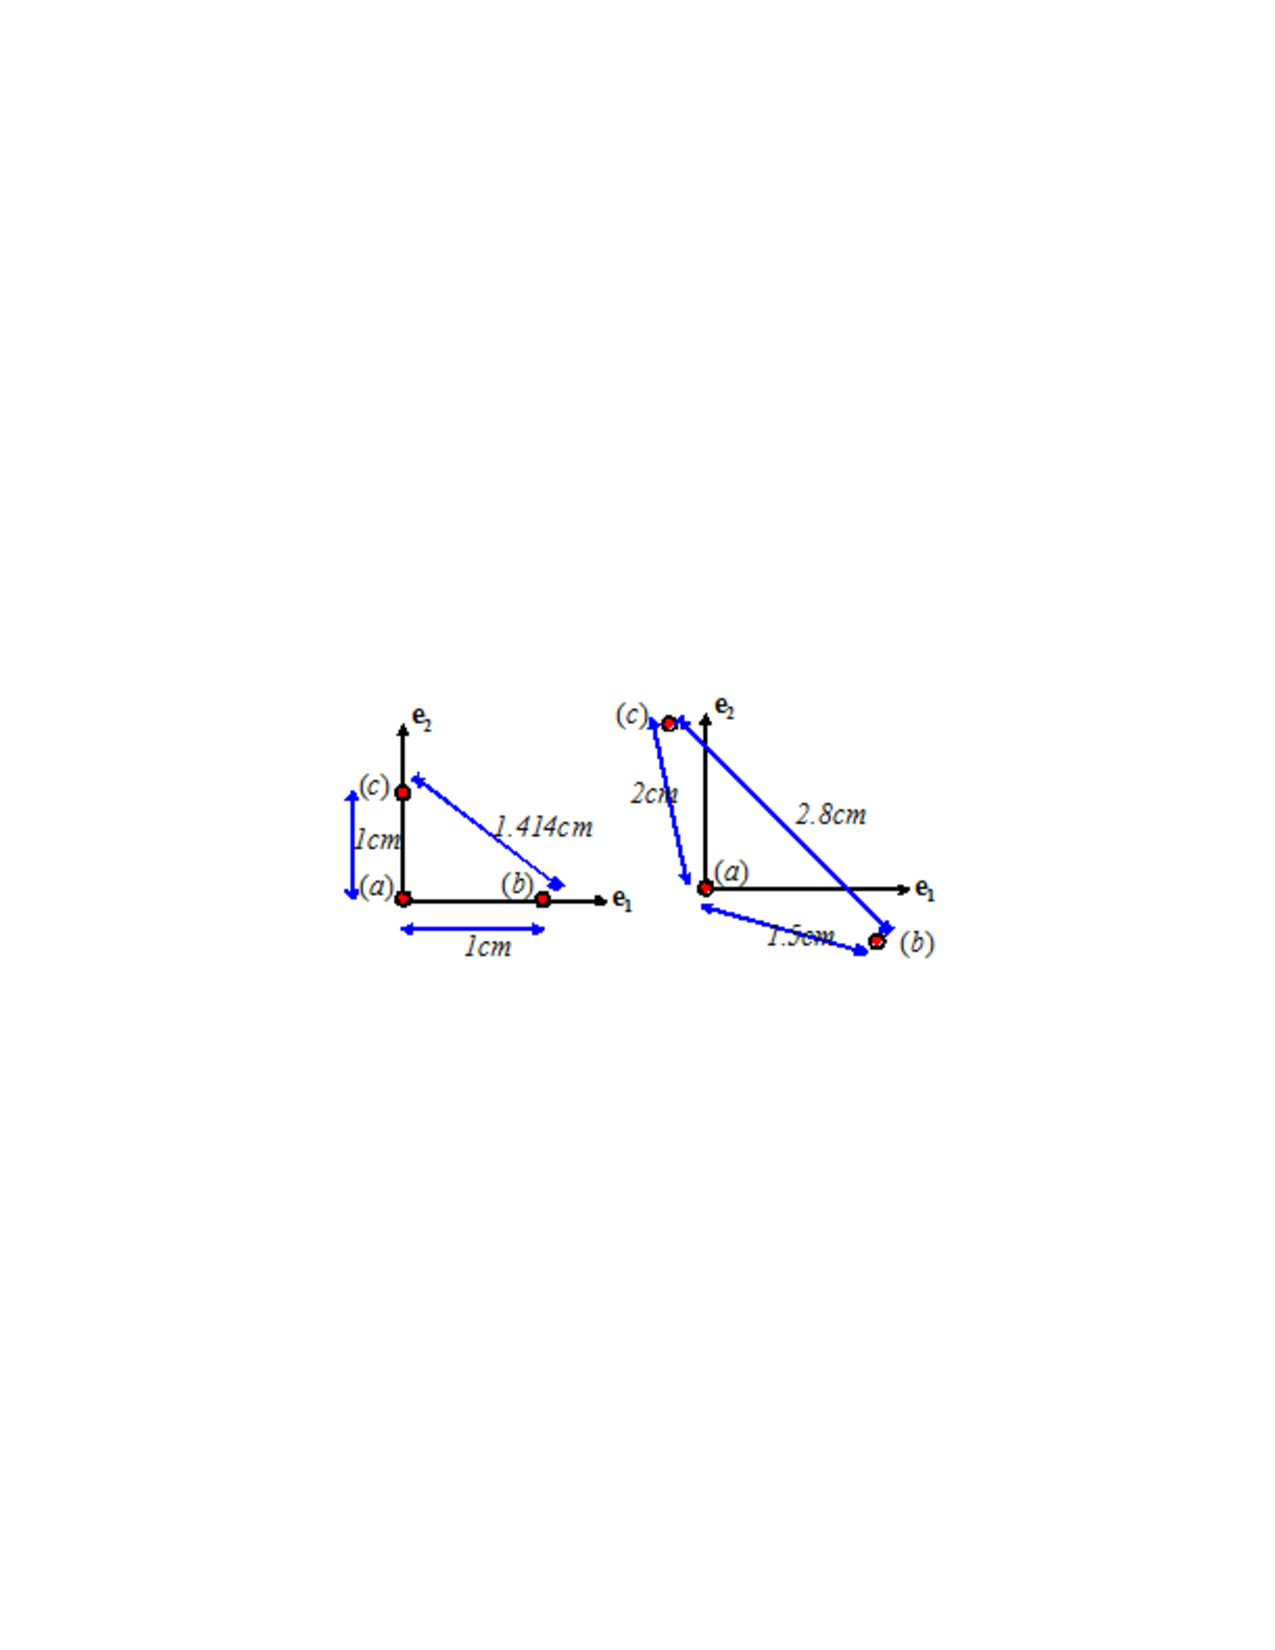
\includegraphics[scale=.6]{INDENT}
\end{center}
%\caption{The considered continuum $\Omega$}
\label{continuum}
\end{figure}

\end{document}